\documentclass{article}
\usepackage{graphicx}
\begin{document}
\hfill Alejandro Chavez

\hfill Lab 2 - Digital Logic

\hfill \today \\
\begin{center}
\begin{large}
Lab 2 - Adding Stuff Up
\end{large}
\end{center}
\begin{itemize}
  \item Part 1 - One Bit Half Adder
  \begin{enumerate}
    \item
      \begin{tabular}{|c|c||c|c|}
        \hline
        A & B & Cout & Sum \\ \hline
        0 & 0 & 0 & 0\\
        0 & 1 & 0 & 1\\
        1 & 0 & 0 & 1\\
        1 & 1 & 1 & 0\\ \hline
      \end{tabular}
    \item
      $Sum\equiv (A\lor B)\land \lnot(A\land B)$\\
      $Cout\equiv (A\land B) $
    \item \textit{One Bit Half Adder}\\ 
      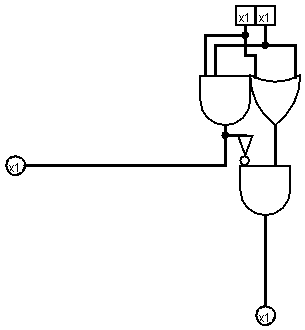
\includegraphics[scale=0.5]{onebithalfadder.png} 
  \end{enumerate}
  \item Part 2 - One Bit Full Adder
  \begin{enumerate}
    \item 
      \begin{tabular}{|c|c|c||c|c|}
        \hline
        A & B & Cin & Cout & Sum \\ \hline
        0 & 0 & 0   & 0    & 0\\
        0 & 0 & 1   & 0    & 1\\
        0 & 1 & 0   & 0    & 1\\
        0 & 1 & 1   & 1    & 0\\
        1 & 0 & 0   & 0    & 1\\
        1 & 0 & 1   & 1    & 0\\
        1 & 1 & 0   & 1    & 0\\
        1 & 1 & 1   & 1    & 1\\ \hline
      \end{tabular}
    \item
    $Sum\equiv (\lnot A\land \lnot B\land Cin)\lor 
    (\lnot A\land B\land \lnot Cin)\lor
    (A\land \lnot B\land \lnot Cin)\lor
    (A\land B\land C)$\\
    $Cout\equiv (B\land Cin)\lor(A\land Cin)\lor (A\land B)$
    \item \textit{One Bit Full Adder}\\
      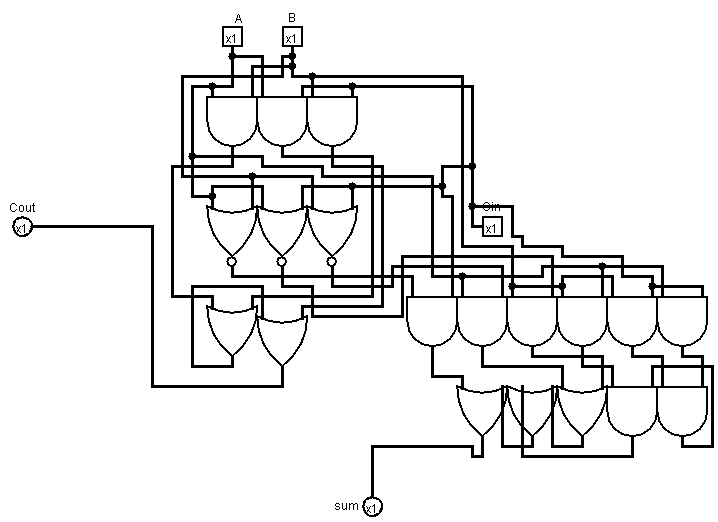
\includegraphics[scale=0.5]{onebitfulladder.png}
  \end{enumerate}
  \item Part 3 - 4-bit Adder
   \begin{enumerate}
    \item \textit{Four Bit Adder}\\
      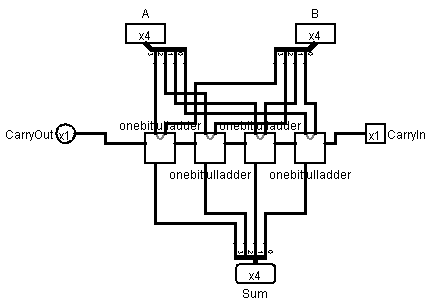
\includegraphics[scale=0.5]{4bitadder.png}
   \end{enumerate}
  \item Part 4 - Logisim 4-bit Adder
    \begin{enumerate}
      \item \textit{Logisim Four Bit Adder}\\
      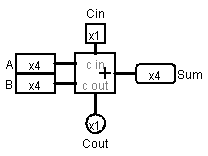
\includegraphics[scale=0.5]{logisim4bitadder.png}
    \end{enumerate}
  \item Questions about a 4-bit Adder
    \begin{enumerate}
      \item
        $0_{10} to 15_{10}$
      \item \textit{4-bit adder table:}
        \begin{center}
        \begin{tabular}{|c|c|c|c|c|c|c|}
          \hline
          Bin. A input & 
          Bin. B input & 
          Bin. sum & 
          Dec. A input & 
          Dec. B input &
          Dec. Sum &
          Carry\\ \hline
          0000 & 0111 & 0111 & 0  & 7  & 7  & 0 \\
          1100 & 0101 & 0001 & 12 & 5  & 17 & 1 \\
          0101 & 0101 & 1010 & 5  & 5  & 10 & 0 \\
          0111 & 1111 & 0110 & 7  & 12 & 22 & 1 \\
          0010 & 0110 & 1000 & 2  & 6  & 8  & 0 \\ \hline
        \end{tabular}
        \end{center}
      \item The only constraint are that the inputs can only be 4 bit unsigned integers, and because of this the circuit will always produce a result that is meaningful considering that there is also a carry out bit.
      \item The carry out pin signifies the 5th bit in the sum.
      \item The four bit adder will use the carry out pin as the "fifth bit" for the sum.
    \end{enumerate}
    
\end{itemize}

\end{document}
